The source model used for this test case comprises a simple vertical strike-slip fault using a truncated Gutenberg-Richter magnitude-frequency distribution (MFD).\\

\noindent Details of the source model are listed below:\\

\noindent
Fault type: Strike slip\\
Fault dip: $90^{\circ}$\\
Fault plane depths: 0--12 km\\
Fault coordinates:\\
South end: $38.0000^{\circ} N$, $122.0000^{\circ} W$\\
North end: $38.2248^{\circ} N$, $122.0000^{\circ} W$\\
Rupture aspect ratio: 2.0\\
Rake angle: $0^{\circ}$\\
Magnitude scaling relationship: Wells and Coppersmith (1994)\\
Magnitude-frequency distribution:\\
Truncated Gutenberg-Richter: $a = 3.1292$; $b = 0.9$; $M_{min} = 5.0$; $M_{max} = 6.5$\\

The time period for both the hazard and the risk calculations in this case are one year. This case uses a collection of 100,000 stochastic event sets, each spanning one year, to generate a set of ground motion fields representative of the seismicity of the specified region, collectively spanning a period of 100,000 years. A single stochastic event set (SES) may contain zero or more ruptures that are generated based on the frequency distribution of the sources. Each SES in this case represents one simulation of the possible events that might occur in one year.

Table~\ref{tab:vf-ln-tax1-zcov} shows the mean loss ratios and corresponding coefficients of variation in the lognormal vulnerability function used in this case. There is no uncertainty in the vulnerability function used for this case. The coefficient of variation of the loss ratio is zero at all intensity measure levels. The purpose of this case is to test the correct interpolation of the mean loss ratios of the vulnerability function at intermediate intensity measure levels and verify the steps involved in the computation of the asset loss exceedance curve and average annual loss.

The hazard calculation produces 4,115 ruptures over the 100,000 cumulative time span, and 4,115 corresponding ground motion fields. The ground motion values at the location of the single asset are $[0.074, 0.154, 0.118, 0.203, \dots, 0.288] g$ (4,115 ground motion values in total).

The calculation of the loss ratios given the ground motion values proceeds in exactly the same manner as described in the Scenario Risk calculator examples. The mean loss ratio and coefficient of variation of the loss ratio are obtained by linear interpolation from the provided vulnerability model for each of the above 4,115 ground motion values. Particularly in this case, since there is no variability in the loss ratio, calculation of the loss ratios for each ground motion field is straightforward. Since the coefficients of variation in the vulnerability function are all zero, the lognormal distribution devolves into the degenerate distribution. Thus, the sampled loss ratio at a particular ground motion intensity level is always equal to the mean loss ratio at that intensity level obtained through interpolation.

These numbers are multiplied by the asset value of $10,000$ to give 4,115 sampled loss values: $[148.90, 308.60, 236.14, 408.76, \dots, 665.79]$ (4,115 loss values in total). This set of losses forms the event loss table (ELT) for the asset.

For the computation of the asset loss curve, the range of loss spanning the minimum and maximum loss observed in the ELT is divided into a number of equispaced intervals as specified by the parameter `loss\_curve\_resolution'. In this case, a value of ten is used for the `loss\_curve\_resolution' parameter. The maximum loss observed in the ELT is $9,713.29$, and the minimum loss observed is $0$. The loss curve is thus calculated at the following eleven points: $[0.00, 1079.25, 2158.51, 3237.76, 4317.02, 5396.27, 6475.53, 7554.78, 8634.03, 9713.29]$.

At each of the eleven loss values on the loss curve, the annual frequency of exceedance of that loss value is obtained by counting the number of ruptures in the ELT which produce losses greater than that loss value, and dividing the count by the cumulative time span of 100,000 years. The loss exceedance counts for the eleven loss values shown above are: $[4030, 799, 293, 133, 87, 48, 25, 13, 6, 0]$. Dividing these exceedance counts by 100,000 gives the corresponding annual exceedance rates or frequencies: $[4.030\times10^{-2}, 7.990\times10^{-3}, 2.930\times10^{-3}, 1.330\times10^{-3}, 8.700\times10^{-4}, 4.800\times10^{-4}, 2.500\times10^{-4}, 1.300\times10^{-4}, 6.000\times10^{-5}, 0.000]$.

Finally, the probabilities of exceedance for the set of eleven loss values are calculated from the annual frequencies of exceedance $\lambda_{L \geq l}$ and the exposure time period $t_R$ through:

\begin{equation}
	prob(L \geq l, t_R) = 1 - \exp (-\lambda_{L \geq l} \times t_R)
\end{equation}

The probabilities of exceedance for the eleven loss values are computed to be the following: $[3.950\times10^{-2}, 7.958\times10^{-3}, 2.926\times10^{-3}, 1.329\times10^{-3}, 8.696\times10^{-4}, 4.799\times10^{-4}, 2.500\times10^{-4}, 1.300\times10^{-4}, 6.000\times10^{-5}, 0.000]$.

The implementation of the event based risk calculator in Julia begins with the set of ground motion fields produced by the OpenQuake event based hazard calculator, and proceeds according to the steps listed above. The loss curve thus calculated above using Julia is compared with the loss curve obtained using the OpenQuake event-based risk calculator in Figure~\ref{fig:lc-ebr-1a}.

\begin{figure}[htbp]
\centering
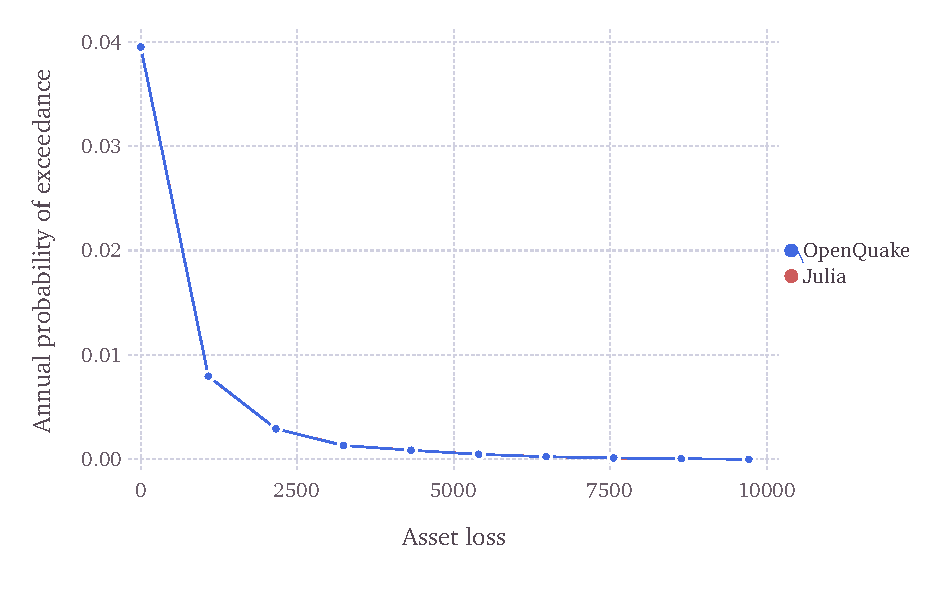
\includegraphics[width=12cm]{qareport/figures/fig-lc-ebr-1a}
\caption{Loss curve comparison for event based risk test case 1a}
\label{fig:lc-ebr-1a}
\end{figure}

The area under the annual loss exceedance curve gives the average annual loss.